\documentclass[compress,t]{beamer}
\usetheme{Custom}
\usepackage{tipa}
\usepackage{tikz}
\usepackage{tabularx}
\usepackage{pgfplots}
\usepackage{enumerate}
\usepackage[caption=false]{subfig}
\usepackage{xcolor,colortbl}

\usepackage{url}

\usepackage{ amsmath, amssymb, lettrine} % don't load graphicx package again -- beamer already does that

\usetikzlibrary{shapes,arrows,calc,patterns,decorations.markings,shadows.blur}
\pgfmathdeclarefunction{gauss}{2}{%
    \pgfmathparse{1/(#2*sqrt(2*pi))*exp(-((x-#1)^2)/(2*#2^2))}%
}

\author{Paul Bienkowski}
\title{Saliency Maps}
\date{2014-07-14}
\institute{Seminar ``Brain Modelling''}


\AtBeginSection[]{
%\newcommand{\sectiontoc}{
    \begin{frame}{\textbf{\insertsectionhead}}
        \tableofcontents[current]
    \end{frame}

    \addtocounter{framenumber}{-1}% If you don't want them to affect the slide number
}

\definecolor{dorsal}{HTML}{BBF7BE}
\definecolor{ventral}{HTML}{DFCDF7}

\begin{document}

\begin{frame}
    \titlepage
\end{frame}

\begin{frame}
    \frametitle{Outline}
    \tableofcontents
\end{frame}

\section{Introduction}
\subsection{Motivation and Definitions}

\begin{frame}{Introduction}
    \begin{figure}[!h]
        \centering
        \begin{tikzpicture}
            \node[anchor=south west,inner sep=0] at (0,0) {
                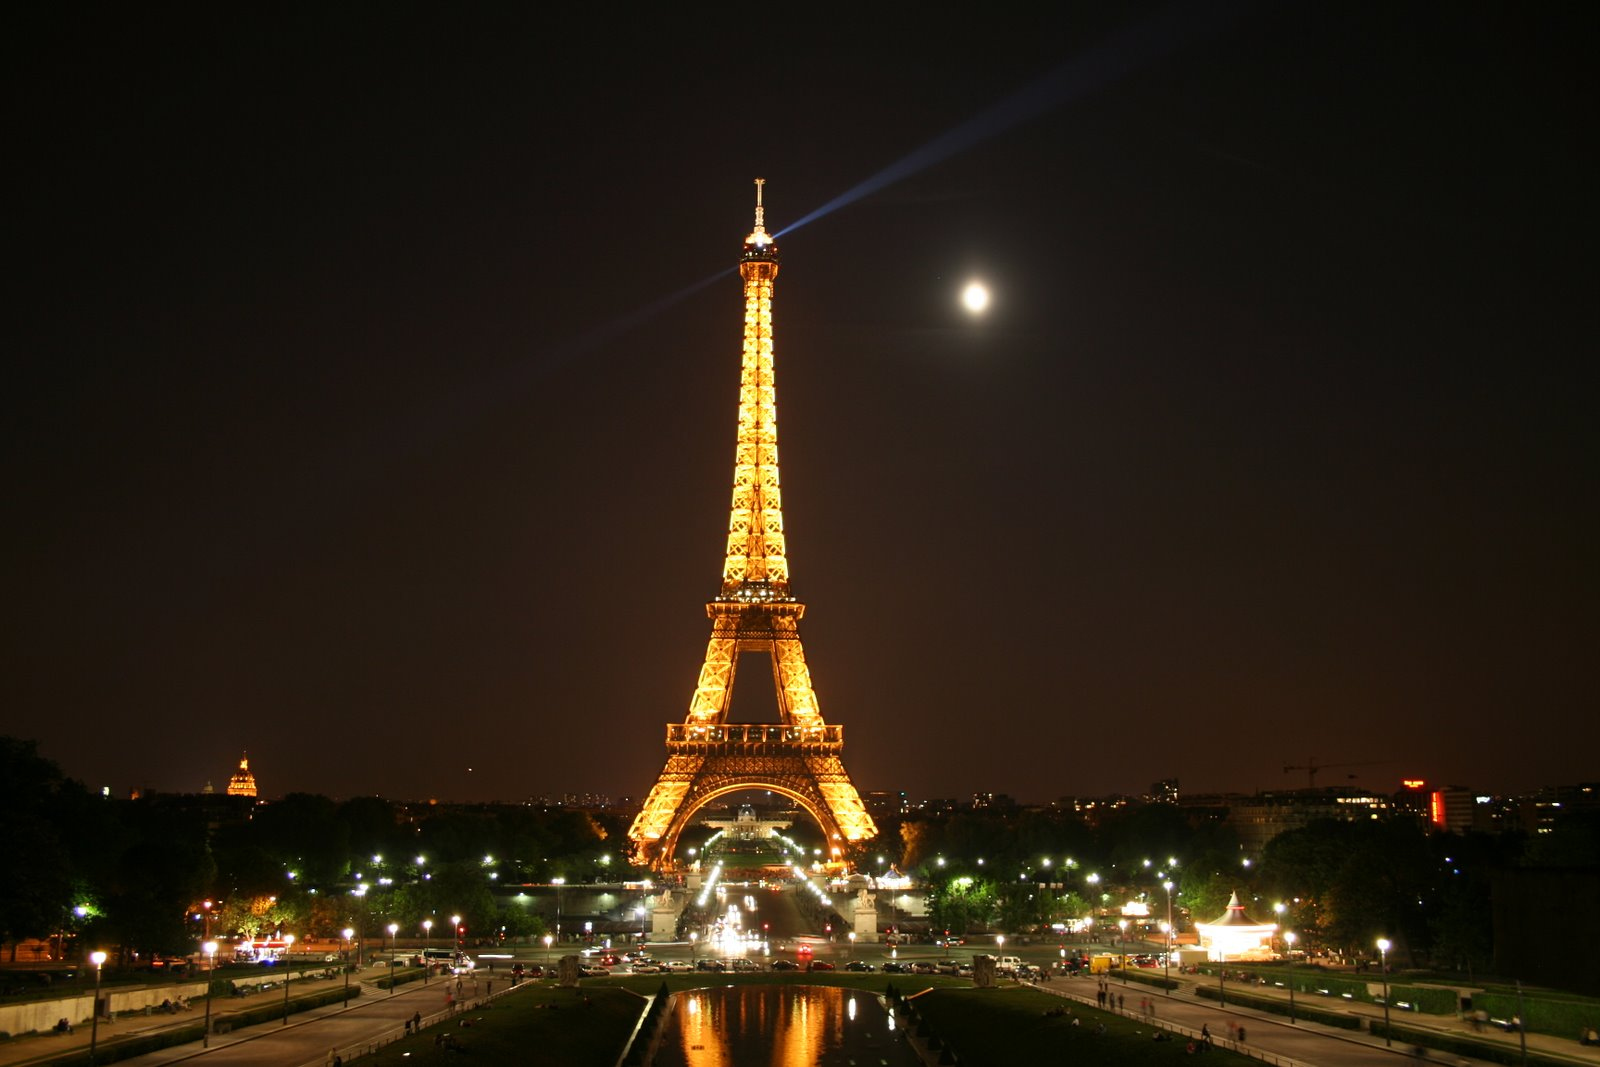
\includegraphics[width=0.9\textwidth]{graphics/eiffel-tower.jpg}
            };

            \draw<2>[red,thick,rounded corners] (8.5,5) rectangle(9.0, 3);

            \draw<3>[green,thick,rounded corners] (3.3,0.5) rectangle (5.8, 5.5);
        \end{tikzpicture}
        \label{fig:eiffel-tower}
    \end{figure}
\end{frame}

\begin{frame}{Introduction}
    \begin{definition}
        \textbf{salient}

        most noticeable or important
    \end{definition}

    \pause

    \begin{definition}
        \textbf{map}
        
        topographically arranged representation of information in a
        multidimensional space
    \end{definition}

    \pause

    \begin{definition}
        \textbf{saliency map}

        A 2D map representing visual saliency of a corresponding visual scene.
    \end{definition}
\end{frame}

\begin{frame}{Motivation}
    \textbf{Biological}
    \begin{itemize}
        \item plan eye movement
        \item see things ``from the corner of the eye''
    \end{itemize}

    \textbf{Technical}
    \begin{itemize}
        \item pre-select important areas from images for image processing
        \item performance gain in computer vision applications
        \item object detection (computer graphics application)
    \end{itemize}
\end{frame}

\begin{frame}<1>[label=examples]{Example Maps}
    \begin{figure}
        \begin{tikzpicture}
            \node[anchor=south west,inner sep=0] at (0,0) {
                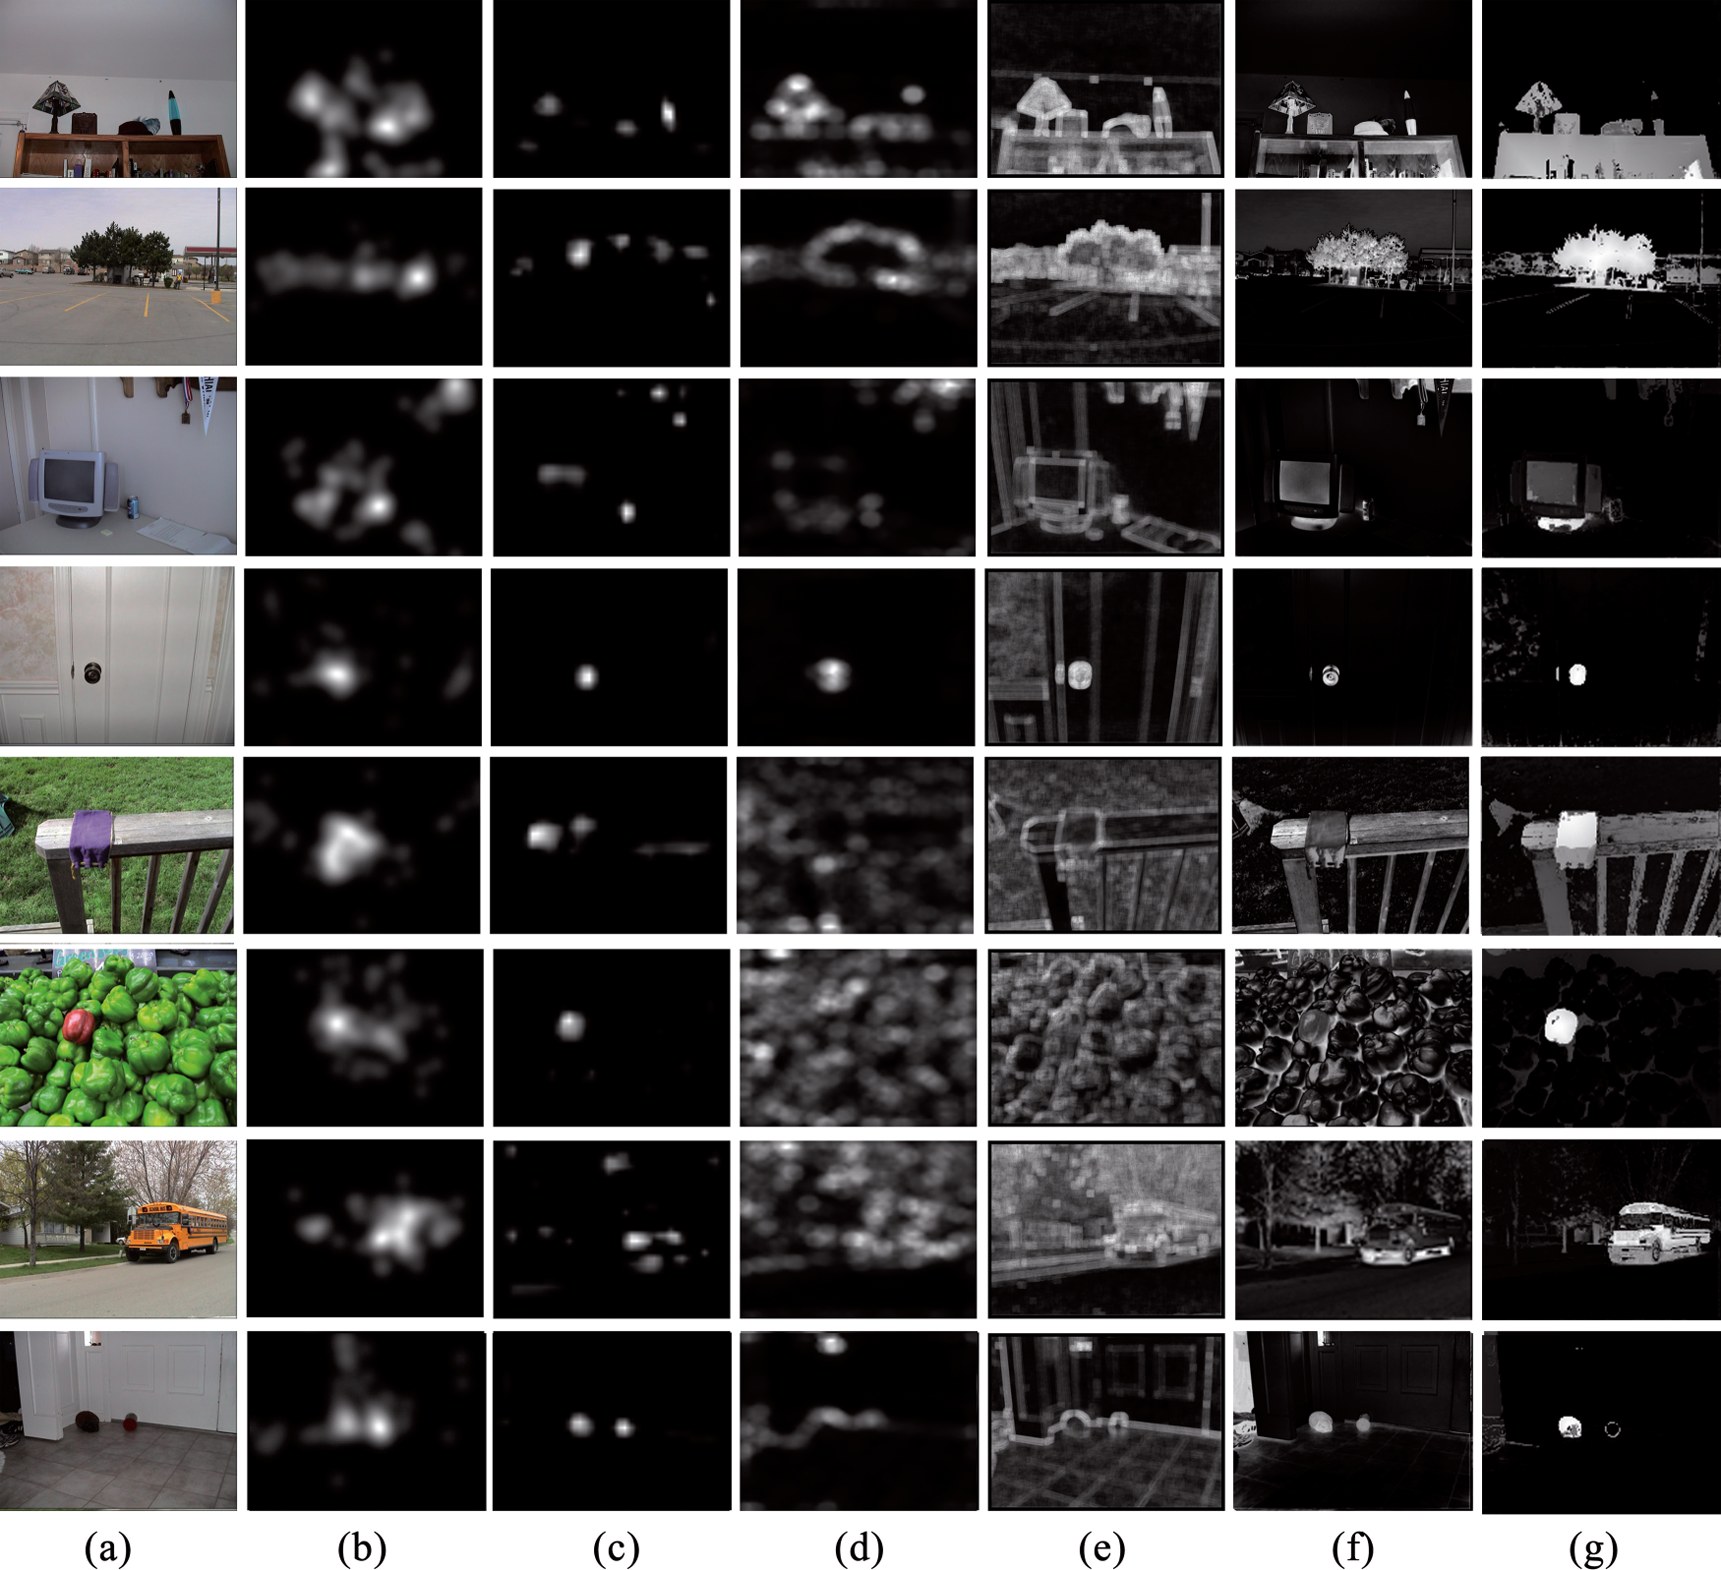
\includegraphics[width=7cm]{graphics/example-maps.png}
            };

            \draw<2>[primary,very thick] (1, -0.05) rectangle(2, 6.4);
            \draw<3>[primary,very thick] (6, -0.05) rectangle(7, 6.4);
            \draw<4>[primary,very thick] (3, -0.05) rectangle(4, 6.4);
        \end{tikzpicture}
        \label{fig:example-maps}
    \end{figure}
\end{frame}

\section{Prequisites}

\subsection{Contrast}
\begin{frame}{Contrast}
    \begin{itemize}
        \item \emph{Color intensity contrast} is the difference in color perception
        \item distance within \emph{Lab color space} \\$\rightarrow$ models perception better than RGB
        \item requires reference color
        \begin{itemize}
            \item global average $\rightarrow$ global contrast
            \item local average function $\rightarrow$ spatial contrast
        \end{itemize}
    \end{itemize}

    \pause



    \textbf{Types of contrast}

    \begin{flalign*}
        \left.
        \begin{minipage}{4cm}
        \begin{itemize}
            \item color
            \item intensity
            \item motion
            \item orientation
            \item depth
        \end{itemize}
        \end{minipage}
        \right\} \text{differences}
    \end{flalign*}
\end{frame}

\subsection{Ventral/dorsal pathway}
\begin{frame}{Ventral/dorsal pathway}

    \begin{figure}
        \centering
        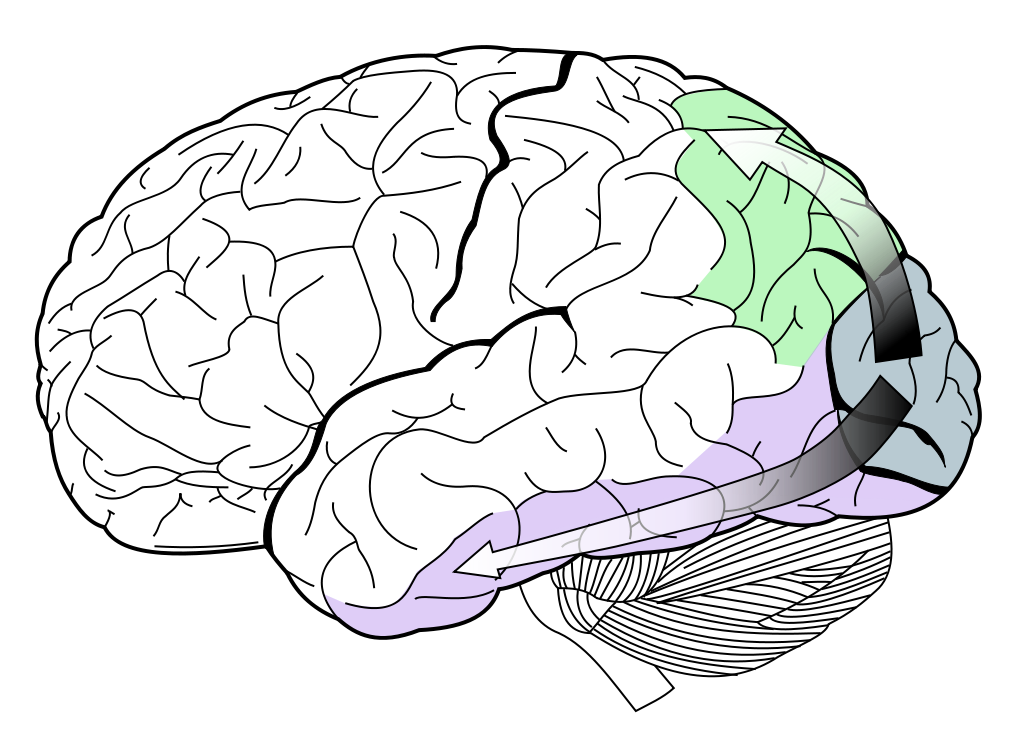
\includegraphics[width=0.5\textwidth]{graphics/ventral-dorsal.png}
        \caption{Ventral and dorsal stream}
        \label{fig:ventral-dorsal}
    \end{figure}

    \scriptsize
    \begin{tabularx}{\textwidth}{|>{\columncolor{ventral}}X|>{\columncolor{dorsal}}X|}
        \hline
        \cellcolor{ventral!70!black}\textcolor{white}{\textbf{What?}} & \cellcolor{dorsal!70!black}\textcolor{white}{\textbf{Where?}} \\ \hline
        Object recognition / identification & Spatial processing \\
        Temporal cortex & Parietal cortex \\
        Ventral stream & Dorsal stream \\ \hline
    \end{tabularx}
\end{frame}

\section{Models and algorithms}

\subsection{Koch/Itti et al. 1987/2001}

\begin{frame}{Koch et al. 1987}{Shifts in selective visual attention: towards the underlying neural circuitry}
    \begin{itemize}
        \item How to handle large amounts of sensory data?
        \item $\rightarrow$ only process parts of them: \textsc{selective attention}
    \end{itemize}

    \pause

    \begin{itemize}
        \item decomposition into early representation of basic features
        \item retinotopical feature maps
        \item combined into one general saliency map
    \end{itemize}

    \pause

    \begin{quote}
        ``A `saliency map`, that is, an explicit two-dimensional topographical map that
        encodes stimulus conspicuity, or saliency, at every location in the visual
        scene.''\cite{itti2001}
    \end{quote}
\end{frame}

\begin{frame}{Koch et al. 1987}{The saliency map}
    \begin{figure}
        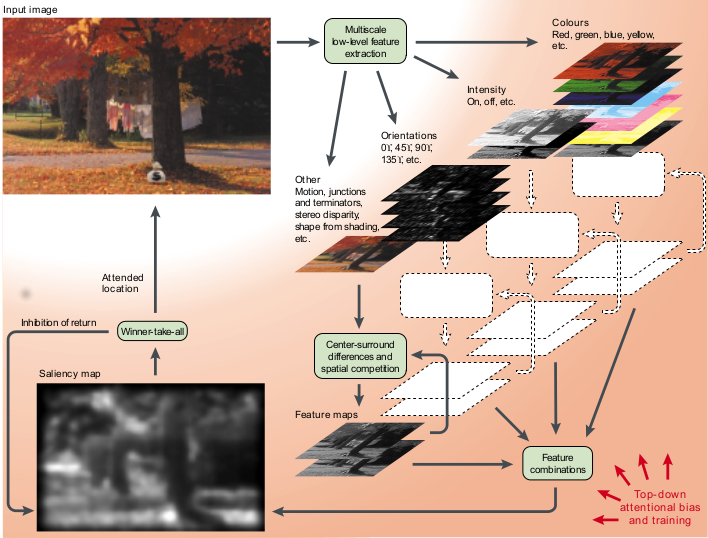
\includegraphics[width=0.85\textwidth]{graphics/koch-maps.jpg}
        \caption{Saliceny map schema}
        \label{fig:koch-schema}
    \end{figure}
\end{frame}

\begin{frame}{Koch et al. 1987}{The saliency map}
    \begin{figure}
        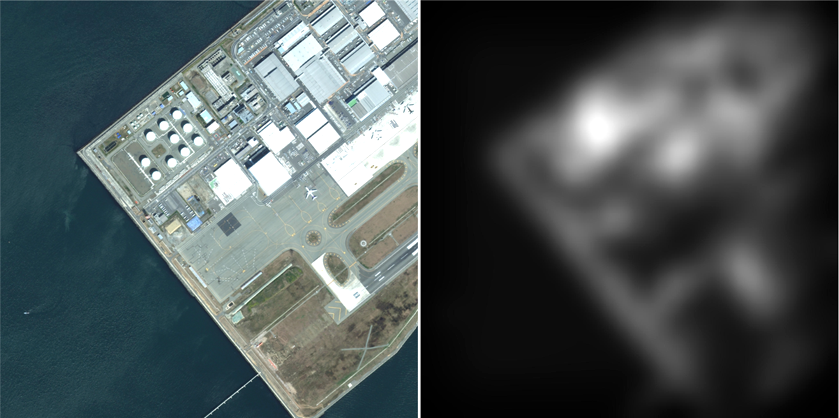
\includegraphics[width=0.9\textwidth]{graphics/koch.png}
        \caption{Sample Koch/Itti saliency map}
        \label{fig:koch-example}
    \end{figure}
\end{frame}

\againframe<2>{examples}

\begin{frame}{Koch et al. 1987}{Visual search}
    To search a visual scene, the saliency map and two mechanisms are required: 

    \pause

    \textbf{Winner-take-all}
    \begin{itemize}
        \item maximum value and location are determined
        \item using complex pyramid-shaped neural network 
        \item directs the next saccade
    \end{itemize}

    \pause

    \textbf{Inhibition of return}
    \begin{itemize}
        \item concept to prevent going back to seen locations
        \item simple to implement using inhibitory synapses
    \end{itemize}
\end{frame}

\begin{frame}{Koch et al. 1987}{Visual search}
    \textbf{Special task:} Search for a person in a group of people

    \begin{itemize}
        \item ventral stream detects faces
        \item feed face locations into saliency map (dorsal stream)
        \item search salient (face) locations for matching face
    \end{itemize}
\end{frame}

\begin{frame}{Itti/Koch et al. 2001}{Computational Modelling of visual Attention}
    \begin{itemize}
        \item Itti refines Koch's model
        \item describes early stages in detail
        \item uses simple localized filters
        \begin{itemize}
            \item center-sourround
            \item gabor kernels
        \end{itemize}
    \end{itemize}

    \pause

    \begin{figure}
        \captionsetup[subfigure]{labelformat=empty}
        \subfloat[\scriptsize Center-sourround / \textsc{Difference of Gaussians}]{
            \begin{tikzpicture}[scale=0.5]
                \begin{axis}[every axis plot/.style={mark=none,domain=-4:4,samples=50,smooth},
                    scale=1,
                    xtick=\empty,
                    ytick=\empty,
                    axis x line*=middle,
                    axis y line*=middle,
                    legend style={legend cell align=right,legend plot pos=right},
                    enlargelimits=true] % extend the axes a bit to the right and top

                    \addplot+[draw=none,
                        mark=none,
                        domain=-0.71:0.71,
                        samples=100,
                        area legend,
                        fill=green!50!white]{gauss(0,0.5)-gauss(0,1)}\closedcycle;
                    \addlegendentry{Excitatory} 

                    \addplot+[draw=none,
                        mark=none,
                        domain=-4:-0.71,
                        samples=100,
                        area legend,
                        fill=red!50!white]{gauss(0,0.5)-gauss(0,1)}\closedcycle;
                    \addplot+[draw=none,
                        mark=none,
                        domain=0.71:4,
                        samples=100,
                        area legend,
                        fill=red!50!white]{gauss(0,0.5)-gauss(0,1)}\closedcycle;
                    \addlegendentry{Inhibitory} 

                    \addplot[dashed] {gauss(0,0.5)};
                    \addplot[dashed] {gauss(0,1)};
                    \addplot[thick] {gauss(0,0.5)-gauss(0,1)};
                \end{axis}
            \end{tikzpicture}
            \label{fig:difference-of-gaussians}
        }
        \hspace{5mm}
        \subfloat[\scriptsize Gabor kernels]{
            \centering
            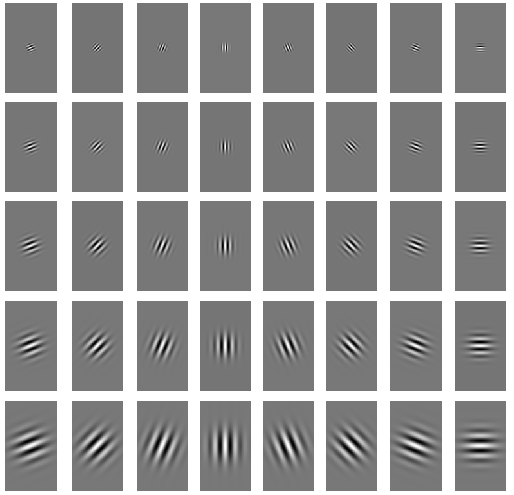
\includegraphics[width=0.3\textwidth]{../paper/gabor-orientations.png}
            \label{fig:gabor-orientations}
        }
    \end{figure}
\end{frame}

\subsection{Perazzi et al. 2012}
\begin{frame}{Perazzi et al. 2012}{Contrast Based Filtering for Salient Region Detection}
    \begin{itemize}
        \item fast and reliable \emph{application-oriented} algorithm
        \item salient \emph{region} detection
        \item contour detail stays intact
    \end{itemize}

    \centering
    \begin{figure}
        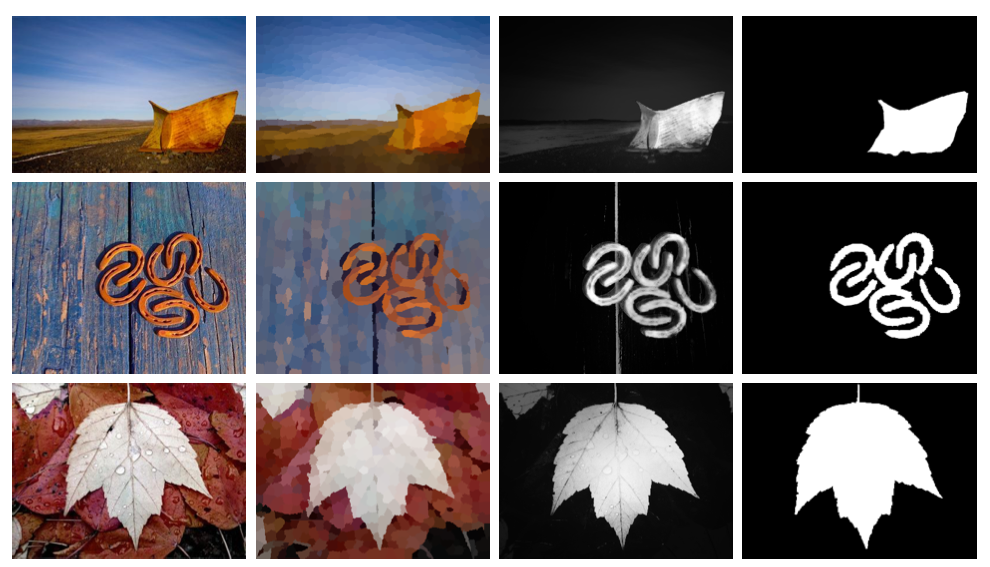
\includegraphics[width=0.7\textwidth]{graphics/example-maps-2.png}
        \label{fig:example-maps-2}
    \end{figure}
\end{frame}

\begin{frame}{Perazzi et al. 2012}{Contrast Based Filtering for Salient Region Detection}
    \begin{enumerate}
        \item segment input image using SLIC
            \begin{itemize}
                \item \emph{Simple Linear Iterative Clustering}
                \item (edge-preserving) K-means clustering algorithms
                \item geodesic image distance in Lab color space
                \item segments are called \emph{elements}
            \end{itemize}
        \pause
        \item analyze segment uniqueness
            \begin{itemize}
                \item rarity of the element color
                \item compared to all other segments
                \item weighted by the distance between them
                \item Gaussian weight function for fast localized uniqueness
            \end{itemize}
        \pause
        \item analyze segment distribution
            \begin{itemize}
                \item occurence of a color elsewhere in the image
                \item low variance $\rightarrow$ compact object $\rightarrow$ more salient
            \end{itemize}
        \pause
        \item combine segment uniqueness and distribution and apply to original pixels
    \end{enumerate}
\end{frame}

\againframe<3>{examples}

\subsection{Hou et al. 2007}
\begin{frame}{Hou et al. 2007}
    \begin{itemize}
        \item in natural scene images, spatial frequency analysis (Fourier transform) yields a typical average pattern
        \item can be used to determine \emph{untypical} frequencies \\ $\rightarrow$ not average image data but interesting object
        \item reverse lookup for saliency map generation
    \end{itemize}
    \pause
    \begin{itemize}
        \item independent of low-level features
        \item filter background noise from data
        \item flexible system
        \item \emph{not neuro-biologically plausible}
    \end{itemize}
\end{frame}

\againframe<4>{examples}

\subsection{Algorithm features}
\begin{frame}{Algorithm features}
    \begin{itemize}
        \item Blurriness
        \begin{itemize}
            \item caused by center-sourround filters or downsampling for performance
            \item no problem in finding single POI\footnote{point of interest} (winner-take-all)
            \item impedes object detection
        \end{itemize}
        \pause

        \item sort POI by intensity
        \begin{itemize}
            \item opposite of boundary detection (binary decision)
            \item required for visual search
        \end{itemize}
        \pause

        \item iterative analysis
        \begin{itemize}
            \item approximate quickly, refine over time
            \item useful in robotics
        \end{itemize}
        \pause

        \item spatio-temporal analysis
        \begin{itemize}
            \item analyze video data, movement detection
        \end{itemize}
    \end{itemize}
\end{frame}


\section{Discussion}

\subsection{Comparison}
\begin{frame}{Comparison}
    \begin{table}[hbt]
        \tiny
        {
        \def\arraystretch{1.5}
        \begin{tabularx}{\textwidth}{lXXX}
        \hline
        \textbf{Approach}
            & \textbf{Itti/Koch} 
            & \textbf{Perazzi}
            & \textbf{Hou} \\ 
        \hline
        Model type
            & neural
            & computational
            & computational \\
        \hline
        Object detection     
            & impossible              
            & great (with contours)
            & good \\
        Sortable by intensity 
            & good / inhibition of return              
            & fair
            & fair \\
        Iterative analysis  
            & simple
            & not possible
            & n/a \\
        Movement detection      
            & use 3-dim. input space
            & possible
            & difficult \\
        \hline
        \end{tabularx}
        }

        \caption{Comparison between approaches and their features and capabilities}
        \label{tbl:comparison}
    \end{table}
\end{frame}

\subsection{Neuro-biological relevance}
\begin{frame}{Neuro-biological relevance}
    \begin{itemize}
        \item Koch/Itti 
        \begin{itemize}
            \item based on neuro-biological findings
            \item easily implementable using feedforward neural networks
            \item combinable with winner-take-all/inhibition of return for visual search
        \end{itemize}    
        \pause
        \item Perazzi \textbf{and} Hou
        \begin{itemize}
            \item computational models
            \item no similar findings in biological research
            \item no obvious neural network implementations
            \item perform tasks associated with both ventral \emph{and} dorsal stream
        \end{itemize}    
    \end{itemize}    

    \pause

    Looking for a neuro-biological model of visual attention? 

    \pause $\Rightarrow$ Koch/Itti!
\end{frame}

\section{Conclusion}
\begin{frame}{Conclusion}
    \begin{itemize}[<+->]
        \item many different saliency detection methods (named three)
        \item either \textbf{neural} or \textbf{computational} models
        \item Koch/Itti is state-of-the-art neuro-biological model for saliency
        \item other algorithms include object detection etc, more task specific
        \item broad area of applications in science and industry
    \end{itemize}
\end{frame}

\section{Appendix}
\begin{frame}[allowframebreaks]{Bibliography}

    \nocite{*}
    \scriptsize
    \bibliographystyle{plain}
    \bibliography{../paper/sources}

\end{frame}

\begin{frame}[allowframebreaks]{Image sources}
    \scriptsize

    \begin{enumerate}
        \item[\ref{fig:eiffel-tower}]
            \url{http://www.npebd.com/wp-content/uploads/2014/06/Eiffel-Tower.jpg}

        \item[\ref{fig:ventral-dorsal}]
            \url{http://upload.wikimedia.org/wikipedia/commons/thumb/f/fb/Ventral-dorsal_streams.svg/1024px-Ventral-dorsal_streams.svg.png}

        \item[\ref{fig:koch-schema}]
            \url{http://cogpsy.info/wp-content/uploads/2012/10/Itti-Koch-2001-Computational-modeling-of-visual-attention.jpg}

        \item[\ref{fig:example-maps}]
            \url{http://opticalengineering.spiedigitallibrary.org/data/Journals/OPTICE/23430/057008_1_9.png}

        \item[\ref{fig:koch-example}]
            \url{http://opticalengineering.spiedigitallibrary.org/data/Journals/OPTICE/24206/OE_51_2_026201_f006.png}

        \item[\ref{fig:gabor-orientations}]
            \url{http://www.intechopen.com/source/html/16592/media/image74.png}

        \item[\ref{fig:example-maps-2}]
            \url{http://stanford.edu/~philkr/imgs/sf_teaser.png}
    \end{enumerate}
\end{frame}

\begin{frame}{Questions?}
    \pause
    \vspace{3cm}
    \centering
    \large{Thanks for your attention!}
\end{frame}

\end{document}